\documentclass[11pt,a4paper]{article}

\usepackage[utf8]{inputenc}
\usepackage[T1]{fontenc}
\usepackage{lmodern}
\usepackage{amsmath}
\usepackage[margin=2.0cm, headheight=14pt]{geometry}
\usepackage{graphicx}
\usepackage{subcaption}
\usepackage{xcolor}
\usepackage{tcolorbox}
\tcbuselibrary{skins,breakable}
\usepackage{enumitem}
\usepackage{fancyhdr}
\usepackage{titlesec}
\usepackage{microtype}
\usepackage{booktabs}
\usepackage{tabularx}
\usepackage{float}
\usepackage[export]{adjustbox}
\usepackage{lastpage}
\usepackage[hidelinks,pdfusetitle]{hyperref}

% Input card macros and graphic search paths
\input{../cardCreation/build/card_macros.tex}
\graphicspath{{../}{../pictures/icons/}{../components/}{images/}{./}}

% Card and Icon rendering macros
\newcommand{\renderCard}[1]{%
  \begin{tikzpicture}
    \node[draw=boxBorder, line width=0.8pt, rounded corners=2.5mm, fill=white, inner sep=0pt] {%
      \resizebox{!}{5.0cm}{#1}%
    };
  \end{tikzpicture}%
}
\newcommand{\inlineIcon}[1]{\raisebox{-0.22ex}{\resizebox{!}{1.15em}{#1}}}

% Color definitions
\definecolor{primaryDark}{HTML}{1A365D}   % Deep navy
\definecolor{accentBlue}{HTML}{2B6CB0}    % Steel blue
\definecolor{arenaRed}{HTML}{C53030}      % Crimson alert
\definecolor{textDark}{HTML}{2D3748}      % Dark charcoal text
\definecolor{boxBg}{HTML}{F8FAFC}        % Light background
\definecolor{boxBorder}{HTML}{CBD5E1}    % Slate border
\definecolor{noteBorder}{HTML}{DD6B20}   % Amber border
\definecolor{noteBg}{HTML}{FFFAF0}       % Amber tint

% Typography & Section formatting
\titleformat{\section}
  {\normalfont\Large\bfseries\color{primaryDark}}
  {\thesection}{0.8em}{}[\color{primaryDark}\titlerule]
\titlespacing*{\section}{0pt}{14pt plus 2pt minus 2pt}{6pt}

\titleformat{\subsection}
  {\normalfont\large\bfseries\color{accentBlue}}
  {\thesubsection}{0.6em}{}
\titlespacing*{\subsection}{0pt}{10pt plus 2pt minus 2pt}{4pt}

\titleformat{\subsubsection}
  {\normalfont\normalsize\bfseries\color{primaryDark}}
  {\thesubsubsection}{0.5em}{}
\titlespacing*{\subsubsection}{0pt}{8pt plus 1pt minus 1pt}{3pt}

% Header and Footer
\pagestyle{fancy}
\fancyhf{}
\fancyhead[L]{\small\color{gray}\textsc{Robot Battles} --- Rules of Play}
\fancyhead[R]{\small\color{gray}Draft Rules}
\fancyfoot[C]{\small Page \thepage\ of \pageref{LastPage}}
\renewcommand{\headrulewidth}{0.4pt}
\renewcommand{\footrulewidth}{0pt}

% Callout box styles
\newtcolorbox{overviewbox}{
  enhanced,
  colback=boxBg,
  colframe=primaryDark,
  arc=2.5mm,
  boxrule=1pt,
  left=10pt,
  right=10pt,
  top=6pt,
  bottom=6pt,
  fontupper=\normalfont
}

\newtcolorbox{draftnotebox}{
  enhanced,
  colback=noteBg,
  colframe=noteBorder,
  arc=2mm,
  boxrule=0.8pt,
  left=10pt,
  right=10pt,
  top=5pt,
  bottom=5pt,
  fontupper=\small\itshape
}

\newtcolorbox{summarybox}[1]{
  enhanced,
  colback=boxBg,
  colframe=accentBlue,
  arc=2mm,
  boxrule=0.8pt,
  title={#1},
  fonttitle=\bfseries\small,
  coltitle=white,
  left=10pt,
  right=10pt,
  top=6pt,
  bottom=6pt
}

\setlist{itemsep=2.5pt, parsep=0pt, topsep=2pt}

\begin{document}

% ==============================================================================
% PAGE 1: OVERVIEW & CARD ANATOMY
% ==============================================================================

\begin{center}
  {\Huge\bfseries\color{primaryDark} Robot Battles}\\[0.3em]
  {\Large\color{accentBlue} Combat Robotics Card \& Miniature Game}\\[0.2em]
  {\normalsize\color{gray} Draft Rules Writeup}
\end{center}
\vspace{0.4em}

\begin{overviewbox}
\noindent\textbf{Theme:} Simple to pick up game to simulate preparing a robot for a competition and fighting it.\\[2pt]
\textbf{Vibe:} Things don't quite work how you want, chaotic, scrambling for fixes and dramatic hits.\\[2pt]
\emph{``You don't know what's going to happen when you enter the box.''}\\[2pt]
\textbf{Design Emphasis:} Game's emphasis is more on making the bot than driving it.
\end{overviewbox}

\vspace{0.2em}

\section{Introduction}

\textbf{Robot Battles} is a game about combat robotics. Build a robot within your budget and weight limit, then defeat your opponents in a tournament of destruction.

\section{Card Anatomy}

Cards represent the physical components, electronics, mechanical assemblies, and weapons installed onto your robot chassis.

\begin{figure}[H]
  \centering
  \begin{subfigure}[b]{0.45\textwidth}
    \centering
    \renderCard{\input{../cardCreation/build/card/Simple_ESC.tex}}
    \caption{Component Card (Electronic Speed Controller)}
    \label{fig:card_esc}
  \end{subfigure}
  \hfill
  \begin{subfigure}[b]{0.45\textwidth}
    \centering
    \renderCard{\input{../cardCreation/build/card/Vertical_Spinner.tex}}
    \caption{Weapon Card (Vertical Spinner)}
    \label{fig:card_weapon}
  \end{subfigure}
  \caption{Card Anatomy and Component Layout}
  \label{fig:card_anatomy}
\end{figure}

The anatomy of each card consists of the following key attributes:

\begin{description}[leftmargin=!, labelwidth=2.8cm, font=\bfseries\color{primaryDark}]
  \item[Price (\$\$):] You cannot have more total price in your pool than your budget.
  \item[Weight:] Your robot's total weight must be less than the weight limit.
  \item[Requirements:] A component is only active if its requirements are supplied by connected components. (Power, spin, pressure are the resources that need supply.)
  \item[Durability:] How much damage a component can take before destruction.
  \item[Absorption:] How much damage a component stops from being passed on during an attack.
  \item[Outputs:] What resources the component supplies. Also includes drive.
  \item[Ability Text:] Any special rules or passive traits for the component.
\end{description}

\vspace{2pt}
\noindent\textbf{Weapon Cards:} Weapon cards will have damage in their output zone, and a template marker indicating which template the component uses and where it attacks (Figure~\ref{fig:card_weapon}).

\clearpage

% ==============================================================================
% PAGE 2: TERMINOLOGY & KEYWORDS
% ==============================================================================

\section{Terminology \& Keywords}

\subsection{Resource Types}

Components produce, require, and consume various resource types. The primary resources used in the game are:

\begin{center}
\renewcommand{\arraystretch}{1.3}
\begin{tabularx}{\textwidth}{c l c X}
  \toprule
  \textbf{Icon} & \textbf{Name} & \textbf{Abbreviation} & \textbf{Description} \\
  \midrule
  \inlineIcon{\resourceE} & \textbf{Energy}   & \texttt{E} & Electrical power generated by batteries, switched by ESCs, and powering motors. \\
  \inlineIcon{\resourceS} & \textbf{Spin}     & \texttt{S} & Rotational kinetic power produced by weapon motors and transferred via belts/pulleys. \\
  \inlineIcon{\resourceP} & \textbf{Pressure} & \texttt{P} & Pneumatic or hydraulic power for actuation and lifters/flippers. \\
  \inlineIcon{\resourceM} & \textbf{Drive}    & \texttt{M} & Motive force delivered to wheels or tracks for arena mobility. \\
  \inlineIcon{\resourceW} & \textbf{Damage}   & \texttt{W} & Destructive impact force dealt to opposing components during active contact. \\
  \bottomrule
\end{tabularx}
\end{center}

\subsection{Resource Notation}

Resources noted on cards follow standardized conventions:
\begin{itemize}
  \item \textbf{Repeated Letter:} Resources noted as repeated letters (e.g., \texttt{EE}) have a symbol drawn for each letter (\inlineIcon{\resourceE}\hspace{1.5pt}\inlineIcon{\resourceE}).
  \item \textbf{Number Followed by Letter:} Resources noted as a number followed by a letter have that number written next to one symbol (e.g., \texttt{6E} is noted as \textbf{6}\hspace{1.5pt}\inlineIcon{\resourceE}).
  \item \textbf{Algebraic Expressions:} The number may also be an algebraic expression (e.g., \texttt{4XW} is noted as \textbf{4X}\hspace{1.5pt}\inlineIcon{\resourceW}). In these cases, the meaning of $X$ is explained in the component's rules text.
\end{itemize}

\subsection{Keywords}

Components may have keywords that define specific mechanical rules and interactions:

\begin{center}
\renewcommand{\arraystretch}{1.45}
\begin{tabularx}{\textwidth}{p{4.0cm} X}
  \toprule
  \textbf{Keyword} & \textbf{Definition / Effect} \\
  \midrule
  \keywordbadge{kw_fragile}{Fragile} & If this component takes weapon damage it is destroyed as if it had a durability of 1. \\
  \keywordbadge{kw_spin_up}{Spin up (X, Y)} & At the start of each turn add X spin counters (max Y) and remove them all if the weapon attacks. \\
  \keywordbadge{kw_forks}{Forks} & If component with forks makes contact and the opponents forks do not make contact, the opponent becomes lifted. \\
  \keywordbadge{kw_wedge}{Wedge} & If this component is hit this robot is not thrown. This effect does not apply if the robot is raised. \\
  \keywordbadge{kw_invertible}{Invertible} & This component works inverted. \\
  \keywordbadge{kw_self_right}{Self-right} & If a turn ends without contact and this robot is inverted, invert it. \\
  \bottomrule
\end{tabularx}
\end{center}

\begin{summarybox}{Keywords Quick Summary}
Keywords provide standardized abilities across components. When evaluating weapon attacks, ground games (forks/wedges), or inversion states, check active component keywords to modify resolution before applying standard damage or throws.
\end{summarybox}

\clearpage

% ==============================================================================
% PAGE 3: ROBOT CONSTRUCTION & THE ARENA
% ==============================================================================

\section{Robot Construction}

Each robot is built onto a chassis. A chassis is a large mat that shows the robot's shape and has a weight, cost, and flip strength. It may have an ability. All cards on the robot must be on the chassis.

\begin{figure}[H]
  \centering
  \begin{subfigure}[b]{0.48\textwidth}
    \centering
    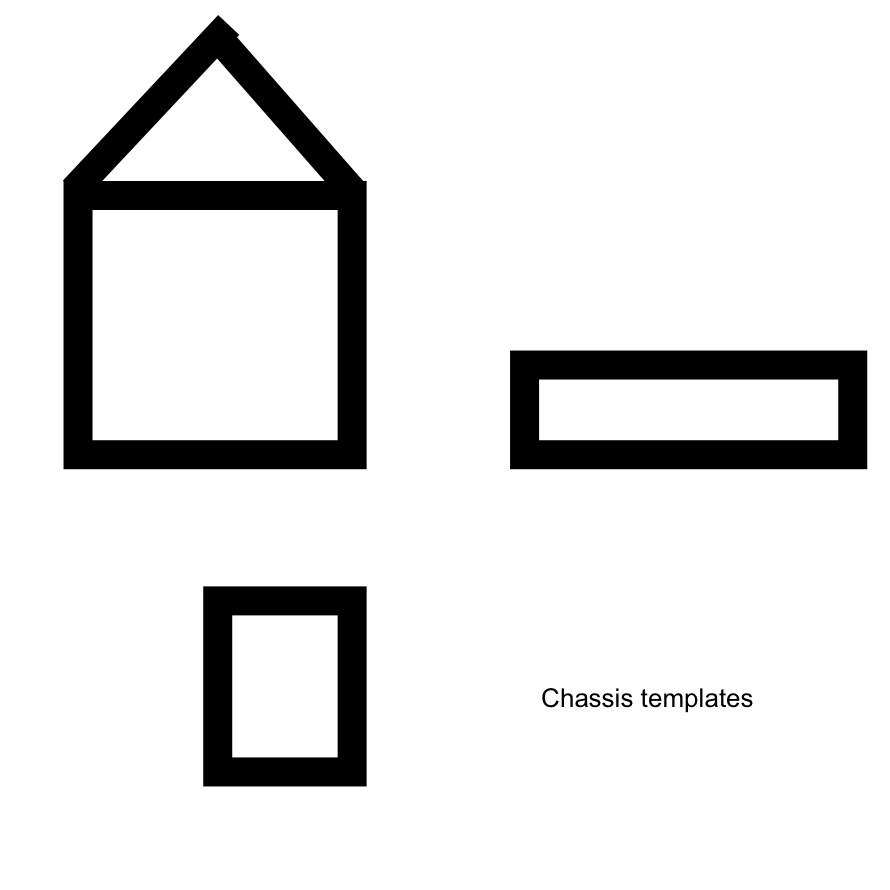
\includegraphics[height=5.2cm]{images/chassis_templates.png}
    \caption{Chassis Templates}
    \label{fig:chassis_templates}
  \end{subfigure}
  \hfill
  \begin{subfigure}[b]{0.48\textwidth}
    \centering
    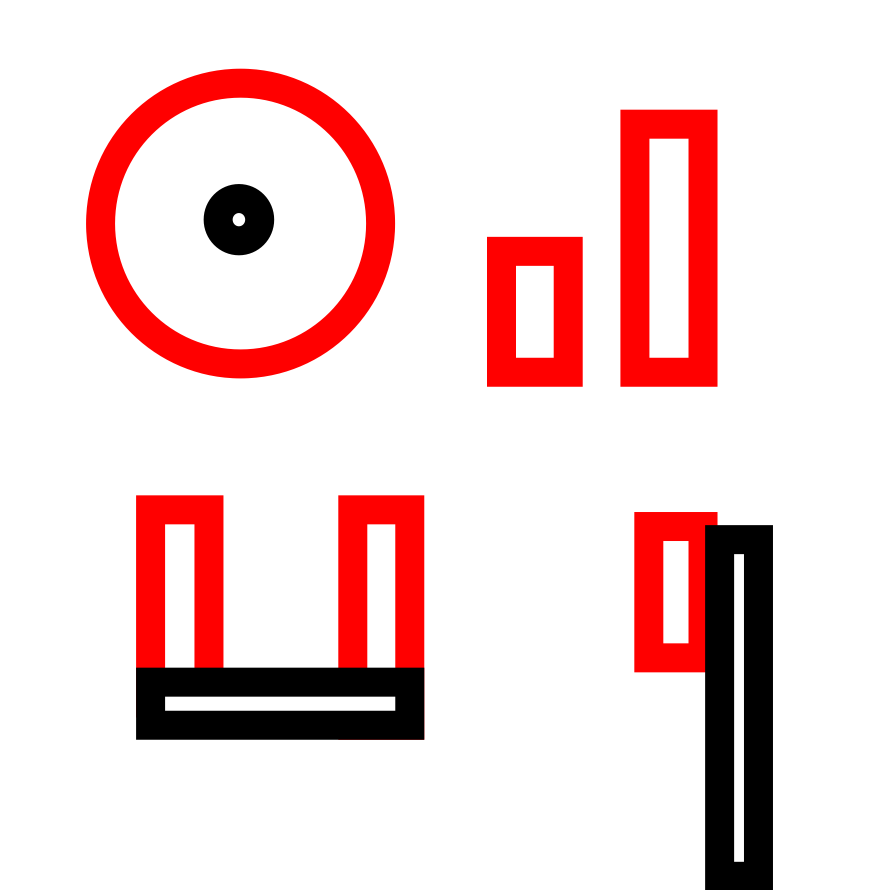
\includegraphics[height=5.2cm]{images/weapon_templates.png}
    \caption{Weapon \& Active Area Templates}
    \label{fig:weapon_templates}
  \end{subfigure}
  \caption{Chassis Shape and Weapon Template Profiles}
  \label{fig:construction_templates}
\end{figure}

\begin{itemize}
  \item The chassis determines the model used for play.
  \item A card is considered connected to any other card it is touching.
  \item You may submit up to two robots, and the total weight across all the robots must be within the weight budget.
  \item Each robot must have active drive to be submitted.
\end{itemize}

\subsection{Resource Supply and Split Supply}

A component is only active if its requirements are supplied by connected components. Supply is resolved on a best-effort basis across connected components: if a component is able to be supplied then it is supplied unless that would mean a higher priority component would become inactive.

Where supply is insufficient to power all connected components, priority is given based on their connected endpoint: drive first, then weapons, unless the robot chose to not use that side's drive this turn (drive = 0). Within the same category it supplies from the largest requirement going down.

If multiple components supply multiple components, sum up and distribute available supply according to the best-effort and priority rules above.

\vspace{0.8em}

\section{The Arena}

Combat takes place inside a hazard-filled enclosed arena.

\begin{figure}[H]
  \centering
  \begin{minipage}[c]{0.44\textwidth}
    \centering
    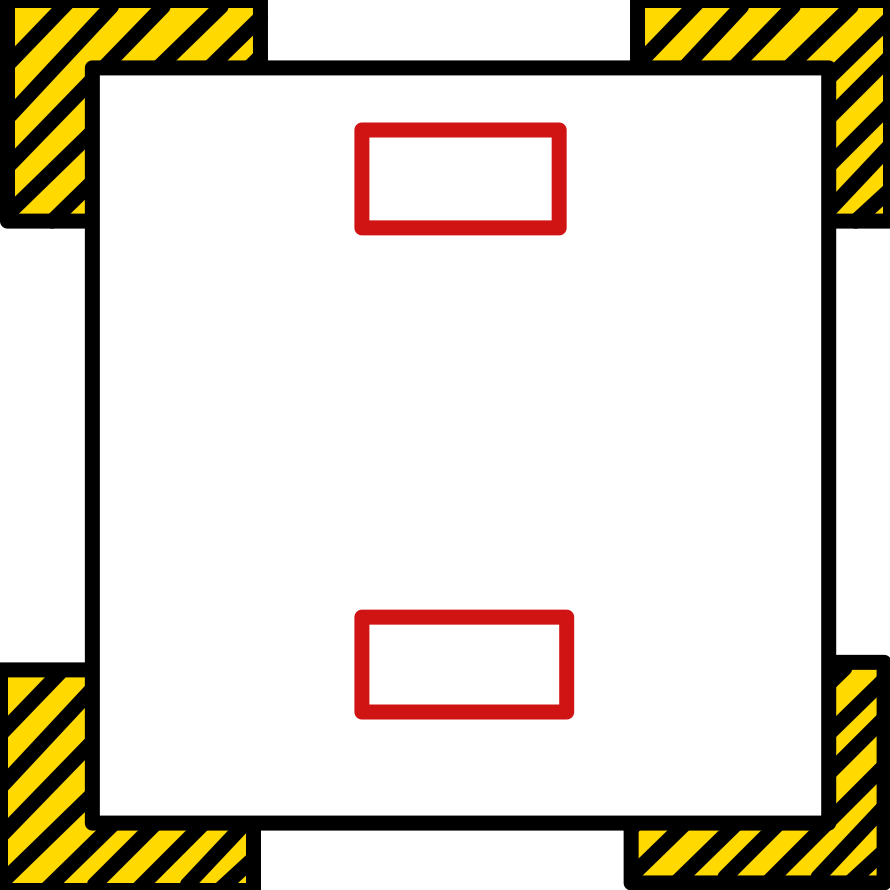
\includegraphics[height=5.8cm]{images/arena_layout.png}
    \caption{The Arena Layout}
    \label{fig:arena}
  \end{minipage}
  \hfill
  \begin{minipage}[c]{0.52\textwidth}
    \textbf{Arena Zones \& Features:}
    \begin{itemize}[leftmargin=*]
      \item \textbf{\color{arenaRed}Red Zone:} Starting area where robots deploy at the beginning of a battle.
      \item \textbf{Black Lines:} Arena perimeter walls. Pushing robots into walls triggers throw feedback.
      \item \textbf{Yellow Hatched:} Arena hazard/pit zones. If a robot is thrown there, they exit the arena and are eliminated.
    \end{itemize}
    \vspace{0.8em}
    \textbf{Robot Markers:}\\
    Each battle starts with both players placing their robot marker (chassis plus weapon --- made from fridge magnets or fancy 3D printed ones) to indicate the position and facing of their robot in the starting zone of the arena.
  \end{minipage}
\end{figure}

\clearpage

% ==============================================================================
% PAGE 4: BATTLE SEQUENCE & MOVEMENT
% ==============================================================================

\section{Battle Rules}
\enlargethispage{2.5\baselineskip}

\subsection{Match Length \& Win Conditions}

The battle is played for \textbf{10 rounds} or until a robot is defeated. A robot is defeated if it has no active drive and no way to uninvert itself to regain drive.

If neither robot is immobilized by the end of round 10, the winner is decided by a \textbf{Judge's Decision}. The judge's decision damage count is the number of cards destroyed followed by the number of cards damaged (the robot with fewer cards destroyed wins; if tied, the robot with fewer cards damaged wins; if still tied, the match is a draw). Total durability is not recorded anywhere in gameplay.

\subsection{Round Structure}

Each round follows a sequence of four phases:

\noindent
{\small\begin{tabularx}{\textwidth}{l p{12.5cm}}
  \toprule
  \textbf{Phase} & \textbf{Summary} \\
  \midrule
  \textbf{1. Planning} & Players secretly select drive settings for each side (absolute value $\le$ active drive count). \\
  \textbf{2. Movement} & Choices are simultaneously revealed; robots advance along the movement templates. \\
  \textbf{3. Collision} & Collisions and contacts (active weapon hits or inert pushes) are resolved. \\
  \textbf{4. Cleanup}  & Reset temporary states, verify active drive, and proceed to the next round. \\
  \bottomrule
\end{tabularx}}

\subsection{Movement Execution}

Movement units are found on the straight movement template. Where an effect says a robot moves that amount, move them along that template without changing facing.

\begin{figure}[H]
  \centering
  \begin{minipage}[c]{0.32\textwidth}
    \centering
    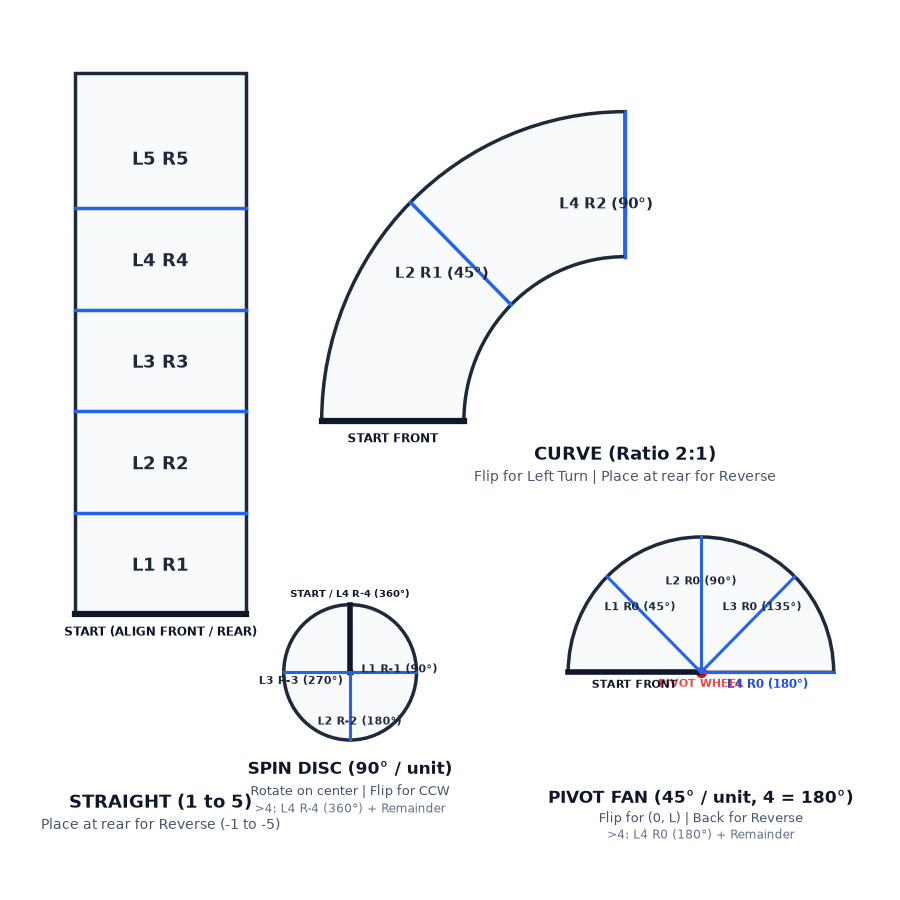
\includegraphics[height=4.3cm]{images/movement_templates.png}
    \caption{Core Templates}
    \label{fig:movement_templates}
  \end{minipage}
  \hfill
  \begin{minipage}[c]{0.65\textwidth}
    \begin{enumerate}[label=\alph*., leftmargin=*, noitemsep, topsep=0.5pt]
      \item In planning, players secretly choose drive settings with absolute value $\le$ active drive count on each side (\texttt{0/0} is stationary). Choices are revealed simultaneously.
      \item Both robots advance along the template corresponding to their chosen drive pair.
      \item \textbf{Forward Alignment:} Front bumper starts flush at black baseline and ends at target line.
      \item \textbf{Left/Right Symmetry (Flipping):} Templates are printed for right turns ($L \ge R$). If turning left ($R > L$), flip the template face-down.
      \item \textbf{Reverse Maneuvers (Rear Placement):} If drive is negative, place the template baseline against the \textbf{back} (rear) of the robot; move backward to the target line.
      \item \textbf{Rotations \& Pivots:} In-place spins ($L = -R$) use the center spin disc in $90^\circ$ increments per unit ($4/-4 = 360^\circ$). Pivots on a locked wheel ($R = 0$ or $L = 0$) use the pivot fan in $45^\circ$ increments per unit ($4/0 = 180^\circ$ semicircle).
      \item \textbf{Movements Beyond the Template:} If drive exceeds markings (e.g., $5/0$, $5/-5$, or boosted drive), move to the template end, then place another template for the remainder.
      \item \textbf{Path Overlap \& Collision Check:} Overlapping paths cause collisions at contact.
    \end{enumerate}
  \end{minipage}
\end{figure}

\vspace{-0.5em}
\begin{summarybox}{Movement Rules Summary}
Drive values chosen in Planning directly determine robot displacement and turning trajectory. Templates cover all 121 permutations with minimal physical pieces: flipping handles left/right turns, placing at the rear handles reverse maneuvers, in-place discs/fans handle rotations, and remainder chaining handles values exceeding template markings.
\end{summarybox}

\clearpage

% ==============================================================================
% PAGE 6: COMPREHENSIVE MOVEMENT EXAMPLES & REFERENCE GUIDE
% ==============================================================================

\subsection{Movement Examples}
\enlargethispage{2.5\baselineskip}

To clarify template usage, physical alignment, and maneuver execution during play, review the following detailed examples:

\vspace{0.2em}
\noindent\textbf{1. Straight Driving and Reverse Maneuvers (\texttt{3/3} vs \texttt{-2/-2})}
\begin{itemize}[leftmargin=*, noitemsep, topsep=1pt]
  \item \textbf{Forward Drive (\texttt{3/3}):} Align Straight Template baseline flush against the \textbf{front bumper}. Advance straight forward until the front bumper aligns with the blue \textbf{L3 R3} line. Heading is unchanged.
  \item \textbf{Reverse Maneuver (\texttt{-2/-2}):} Negative drive moves backward. Align baseline flush against the \textbf{rear bumper} pointing backward. Reverse until the rear bumper aligns with \textbf{L2 R2}. Heading is unchanged.
\end{itemize}

\vspace{0.2em}
\noindent\textbf{2. Curved Arcs and Left/Right Flipping (\texttt{2/1} vs \texttt{1/2})}
\begin{itemize}[leftmargin=*, noitemsep, topsep=1pt]
  \item \textbf{Right Turn Arc (\texttt{2/1}):} Place the 2:1 Curve Template face-up with baseline at the front bumper. Advance along the curve to line \textbf{L2 R1}, sweeping $45^\circ$ clockwise to the right ($\Delta\theta = (2 - 1) \times 45^\circ$).
  \item \textbf{Left Turn Arc (\texttt{1/2}):} Right track is faster ($R > L$), turning left. Take the \textbf{exact same} 2:1 Curve Template and \textbf{flip it face-down}. Advance along the arc to \textbf{L2 R1}, sweeping $45^\circ$ counter-clockwise.
  \item \textbf{Reverse Curve (\texttt{-2/-1}):} Placed face-up against the rear bumper; robot backs up along the curved track.
\end{itemize}

\vspace{0.2em}
\noindent\textbf{3. Pivot Fan vs. Spin Disc Rotations (\texttt{2/0} vs \texttt{2/-2})}
\begin{itemize}[leftmargin=*, noitemsep, topsep=1pt]
  \item \textbf{Pivot on Stationary Wheel (\texttt{2/0}):} Right wheel is locked. Place Pivot Fan red marker on the \textbf{right wheel}. Robot swings clockwise around that wheel by $90^\circ$ ($2 \times 45^\circ$) to line \textbf{L2 R0}.
  \item \textbf{Spin-on-the-Spot (\texttt{2/-2}):} Tracks counter-rotate equally. Center the Spin Disc under the chassis. Robot rotates $180^\circ$ clockwise ($2 \times 90^\circ$) to \textbf{L2 R-2} on the spot with zero displacement.
\end{itemize}

\vspace{0.2em}
\noindent\textbf{4. Movements Beyond the Template (Remainder Chaining: \texttt{5/0}, \texttt{5/-5}, \texttt{6/6})}
\begin{itemize}[leftmargin=*, noitemsep, topsep=1pt]
  \item \textbf{Extended Pivot (\texttt{5/0}):} Pivot Fan markings end at \textbf{L4 R0} ($180^\circ$ semicircle). Pivot to template end at \textbf{L4 R0} ($180^\circ$), then from this new position place the template again for remainder ($5 - 4 = 1$), pivoting an additional $1$ unit (\textbf{L1 R0}, $45^\circ$) for total rotation of $180^\circ + 45^\circ = \mathbf{225^\circ}$.
  \item \textbf{Whirlwind Spin (\texttt{5/-5}):} Spin Disc marks end at \textbf{L4 R-4} ($360^\circ$). Spin $360^\circ$ to template end, then apply remainder ($1$ unit, \textbf{L1 R-1}) to rotate an additional $90^\circ$, completing a total spin of $\mathbf{450^\circ}$.
  \item \textbf{Overdrive Straight (\texttt{6/6}):} Boosted drive past 5 advances to \textbf{L5 R5} at template end, then places template again for remainder \textbf{L1 R1}.
\end{itemize}

\vspace{0.2em}
\noindent\textbf{5. Counter-Drive Tight Turns (\texttt{3/-1})}
\begin{itemize}[leftmargin=*, noitemsep, topsep=1pt]
  \item \textbf{Tight Hook Turn (\texttt{3/-1}):} Track 1 drives forward 3 units while opposing track reverses 1 unit. Uses Tight Turn Template (3:-1 ratio). Counter-rotation with unequal speeds swings robot $180^\circ$ while translating slightly forward.
\end{itemize}

\vspace{0.2em}
\begin{table}[H]
\centering
\small
\renewcommand{\arraystretch}{1.12}
\begin{tabularx}{\textwidth}{l c c X}
  \toprule
  \textbf{Drive Pair} & \textbf{Category} & \textbf{Template Used} & \textbf{Physical Placement \& Execution Rule} \\
  \midrule
  $L = R > 0$ & Straight & Straight (1--5) & Front baseline. Move forward with fixed heading. \\
  $L = R < 0$ & Reverse & Straight (1--5) & Rear baseline. Reverse backward with fixed heading. \\
  $L > R > 0$ & Curve (Right) & Curve Arc & Front baseline, face-up. Turn right by $(L - R)\times 45^\circ$. \\
  $R > L > 0$ & Curve (Left) & Curve Arc & Front baseline, \textbf{flip face-down}. Turn left by $(R - L)\times 45^\circ$. \\
  $L > 0, R = 0$ & Pivot (Right) & Pivot Fan & Red pin on right wheel. Pivot CW by $L \times 45^\circ$ (4 = $180^\circ$). \\
  $L = 0, R > 0$ & Pivot (Left) & Pivot Fan & \textbf{Flip face-down}, pin on left wheel. Pivot CCW by $R \times 45^\circ$. \\
  $L = -R$ & Spin Disc & Spin Disc & Centered under chassis. Spin on spot by $L \times 90^\circ$ (4 = $360^\circ$). \\
  $L > 4$ or $|R| > 4$ & Chaining & Same Template & Move to template end, then apply template again for remainder. \\
  \bottomrule
\end{tabularx}
\caption{Differential Drive Permutation Reference Guide}
\label{tab:drive_ref}
\end{table}

\clearpage

% ==============================================================================
% PAGE 5: COLLISIONS & CONTACT RESOLUTION
% ==============================================================================

\section{Collisions \& Contact Resolution}

\subsection{Determining the Contact Point}

For a collision, first determine which octant of each robot makes contact with the other: place both robots as far along their path as they can go without touching the other's path, then slowly move both forwards until they touch each other. Where the robots touch shows the contact point. Where ambiguous, both components make contact.

\begin{itemize}
  \item \textbf{Active Contact:} If the parts of either robot that is touching is the weapon's active area (the red zone on the template), then the contact is active.
  \item \textbf{Inert Contact:} Otherwise, it is an inert contact.
\end{itemize}

\subsection{Inert Contact (Pushing Match)}

Essentially a pushing match between colliding chassis surfaces:
\begin{itemize}
  \item The pair of robots move in the line drawn between their two centers through the point of contact.
  \item The distance they move is the sum of their remaining motion in that direction: all other distance is lost.
  \item If a robot is pushed into a wall, it is thrown with a throw strength equal to the amount it would have moved if the wall wasn't there.
  \item Each robot takes feedback shared equally between its remaining active drive equal to the remaining distance the opponent had before the contact.
  \item After any inertial contact, separate the robots by moving them both away from each other one step if possible.
\end{itemize}

\begin{draftnotebox}
  \textbf{Editor Note:} [Needs a diagram here]
\end{draftnotebox}

\subsection{Active Contact (Weapon Hits)}

When weapons collide with an opponent's chassis or components:
\begin{itemize}
  \item All weapons involved in the contact are assumed to hit, and they deal damage according to their damage level to the other robot to the components contacted.
  \item Then both robots are thrown away from the contact. The base throw strength is equal to the attack strength received.
  \item Weapons receive feedback equal to half the total attack strength in the contact.
  \item If after active contact the robots are still in contact, then proceed with inertial contact, at the end of which both robots are rotated a random amount.
\end{itemize}

\begin{summarybox}{Contact Classification Quick Reference}
\begin{tabularx}{\textwidth}{l X}
  \textbf{Contact Type} & \textbf{Resolution Mechanism} \\
  \midrule
  \textbf{Active Contact} & Weapon strikes component $\rightarrow$ Deals weapon damage level $\rightarrow$ Base throw strength equals attack strength received $\rightarrow$ Weapons take feedback equal to $\frac{1}{2}\times\text{attack strength}$. If robots are still in contact, proceed with inertial contact (rotating both robots a random amount at the end). \\
  \addlinespace[3pt]
  \textbf{Inert Contact} & Pushing match along line between centers $\rightarrow$ Move sum of remaining motion in that direction $\rightarrow$ Wall collision causes throw $\rightarrow$ Drive takes feedback equal to opponent's remaining distance $\rightarrow$ Separate robots by moving both away from each other 1 step if possible. \\
\end{tabularx}
\end{summarybox}

\clearpage

% ==============================================================================
% PAGE 6: COMBAT RESOLUTION, DAMAGE & STATUS EFFECTS
% ==============================================================================

\section{Combat Resolution, Damage \& Status Effects}

\subsection{Throws \& Inversion}

A robot that is thrown is moved a random amount (2d6) up to the throw strength away from the contact point and rotated by spinning the model. 
If the throw strength minus the thrown distance is greater than the flip value of the chassis, the robot is \textbf{inverted}.
After the throw the thrown robot takes feedback at a randomly chosen component equal to half the throw strength (unless the robot hits a wall, in which case it takes feedback equal to the full throw strength). 
Component is chosen randomly by dropping a card on it.


\subsection{Damage Progression}

Damage progresses from the outermost component inwards, applying absorption at each step until all the damage is absorbed:

\begin{itemize}
  \item \textbf{Component Destroyed:} A component is destroyed if the remaining damage level that hits it exceeds its durability.
  \item \textbf{Component Damaged:} A component is damaged if the remaining damage level minus that component's absorption is greater than half its durability.
  \item \textbf{Repeated Damage:} If a damaged component would be damaged again, it is instead destroyed.
  \item \textbf{Absorption on Destruction:} If a component is destroyed, it absorbs damage equal to its durability instead of its absorption.
\end{itemize}

All damage numbers are integers; when sharing or dividing, round down. Total durability is not recorded anywhere in gameplay; components simply transition between undamaged, damaged, and destroyed.

\subsection{Feedback}

Feedback represents components over-straining themselves under combat loads. It is damage that progresses back from the source component 
to each component that supplies it, shared equally if there are multiple components (rounding down), down the tree until the damage is all absorbed.

\subsection{Status Effects}

\begin{description}[leftmargin=!, labelwidth=2.5cm, font=\bfseries\color{primaryDark}]
  \item[Inverted:] While a robot is inverted, weapons and drive without the \textit{invertible} keyword don't work. If an inverted robot would be inverted again, it becomes the right way up.
  \item[Raised:] Some components (mostly forks) will make the opponent raised if they make contact. A robot that is raised has its drive strength halved for as long as it is in contact with the component that raised it, and its flip strength is halved. The Wedge effect does not apply if the robot is raised.
\end{description}

\begin{summarybox}{Damage \& Feedback Rules Summary}
\begin{itemize}[leftmargin=*]
  \item \textbf{Integer Damage:} All damage numbers are integers; when sharing or dividing, round down.
  \item \textbf{Damage Inward Progression:} Attack Damage $\rightarrow$ Absorbed by outermost layer $\rightarrow$ Excess damage hits next connected internal component.
  \item \textbf{Damage Conditions:} Exceeds durability $\implies$ \textbf{Destroyed}. Exceeds $\frac{1}{2}$ durability after absorption $\implies$ \textbf{Damaged}. Damaged again $\implies$ \textbf{Destroyed}.
  \item \textbf{Throw Damage:} Throw feedback equals half the throw strength (rounded down), unless the robot hits a wall (which inflicts full throw strength).
  \item \textbf{Active into Inertial Contact:} If after active contact the robots are still in contact, proceed with inertial contact, at the end of which both robots are rotated a random amount.
  \item \textbf{Inertial Separation:} After any inertial contact, separate the robots by moving them both away from each other 1 step if possible.
  \item \textbf{Wedge Immunity:} A component with the Wedge keyword prevents the robot from being thrown when hit; this effect does not apply if the robot is raised.
  \item \textbf{Durability in Play:} Total durability is not recorded anywhere in gameplay.
  \item \textbf{Feedback Backward Propagation:} Reverse flow from component back into power/pressure suppliers, distributed equally (rounded down).
\end{itemize}
\end{summarybox}

\clearpage

% ==============================================================================
% PAGE 7: GAME FORMATS & TOURNAMENT PLAY
% ==============================================================================

\section{Game Formats}

\subsection{Preconstructed}

\begin{itemize}
  \item Each player brings a build deck up to the budget chosen (we recommend \$25).
  \item Then you each build a robot from that up to the weight limit and fight with those.
\end{itemize}

\subsection{Limited (Recommended)}

\begin{itemize}
  \item There is a pool in the middle of cards, split into basic and special.
  \item You can grab anything from the basic pile.
  \item For special cards, there is a market of 9 face-up cards you can take from, after which you must reveal the next card. You cannot return any card you have taken to the supply once you have taken it.
  \item You cannot take more total cost than your budget (\$25 recommended).
  \item From this pool, you build your robot to fight with. You are considered to have an infinite supply of all free components.
\end{itemize}

\subsection{Quickstart / Latecomer}

If you just want to dive right into the action, you can grab one of the automaton robot sheets and play using that (in this case, ignore the automation lines).

\subsection{Tournament Play}

\begin{itemize}
  \item \textbf{Format Structure:} Robot Battles is designed to be played across multiple battles (typically 3), where you repair your robot from the spares in your supply between rounds. Components damaged in one round cannot be used in future rounds.
  \item \textbf{Victory Condition:} The winner of the tournament is the player with the most wins after all games are played.
  \item \textbf{Pairings:} Battles are played with random pairings for round 1, then with a ``winners play winners'' pattern. If you have an odd number of players, include an automaton as one person in the tournament (feel free to include more if you like).
\end{itemize}

\subsection{Automaton Robots}

There are some automaton robots which come with a pre-built setup printed on their A3 sheet. You can use dry-erase markers to write on this damage during a fight.

They will take actions according to the table written on the right-hand side of their sheet.
First check the chart to see which table to roll on based on the current state of the robot.
Then roll a d6 to see which action they take.
The possible actions are as follows:
\begin{itemize}
  \item \textbf{Rush:} They will move at maximum speed towards their opponent.
  \item \textbf{Face:} They rotate on the spot to face their opponent.
  \item \textbf{Retreat:} They face towards their opponent and move backwards 1 step.
\end{itemize}
From this you can calculate the drive values that they will choose (for each they consider the current position of their opponent). 
Roll this after deciding your own drive values.


\end{document}
